\section{\texttt{ZIP-FIT}: an Embedding-Free Data Selection Algorithm via Compression-Based Alignment for LM Fine-Tuning}
\begin{figure*}[t]
    \centering
    {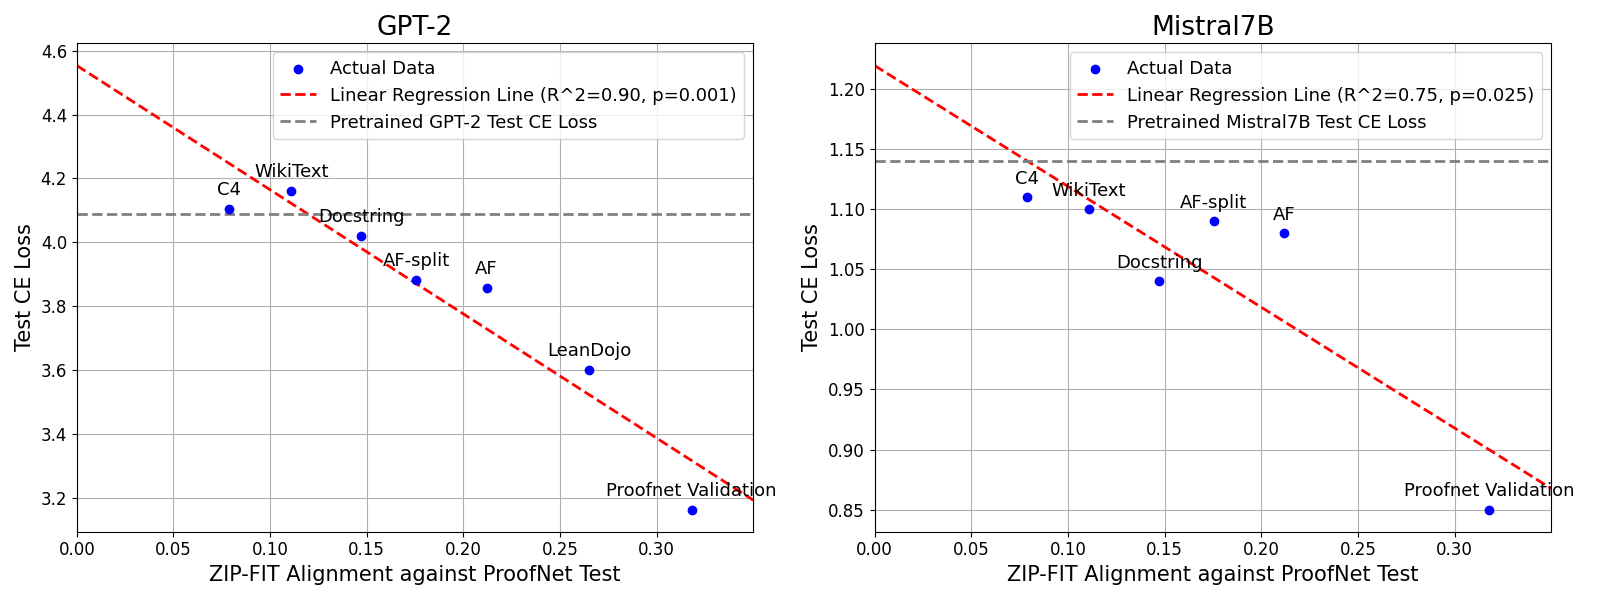
\includegraphics[width=\textwidth]{plots/ce_loss_combined.png}}
    \caption{\textbf{Higher \texttt{ZIP-FIT} alignment correlates with lower cross-entropy loss.} The relationship between \texttt{ZIP-FIT} alignment and cross-entropy (CE) loss for (a) GPT-2 trained on 22k tokens ($R^2 = 0.90, p=0.001$) and (b) Mistral7B trained on 22k tokens ($R^2 = 0.75, p=0.025$). Each point represents a dataset, with its position reflecting the dataset’s \texttt{ZIP-FIT} alignment score against the ProofNet test set and the resulting CE loss. The dashed red line indicates the linear regression fit, while the dashed grey line shows the pretrained CE loss. Higher alignment scores correspond to lower CE losses, demonstrating that training on better aligned data yields better performance.}
    \label{fig:ce_vs_gzip_align}
\end{figure*}
Before introducing \texttt{ZIP-FIT}, it is essential to understand the desired attributes of effective data selection algorithms. Ideally, such algorithms should be performant, computationally economical, fast, scalable, and designed to improve the efficiency of model training. These characteristics ensure that the data filtering process can be applied broadly and effectively in various machine learning contexts, particularly when computational resources are limited. By setting these criteria, we can better appreciate the innovations \texttt{ZIP-FIT} introduces in the realm of data selection.



\subsection{Background}

\textbf{\texttt{gzip} compression}: uses two main techniques for compression, LZ77 and Huffman coding. 
Together, these methods compress sequences by exploiting repeated patterns in the data. 
LZ77 works by identifying repeated substrings and replacing them with references to their earlier occurrences.
Huffman coding further compresses the data by assigning shorter binary codes to more frequent symbols, optimizing the overall length of the compressed text.
For more details, see Appendix~\ref{app:sec:gzip_compression_details}.

\textbf{AutoFormalization (AF):} refers to the task of translating natural language mathematical statements into a formal mathematical programming language, like Lean4 \cite{deMoura2015lean}. 
This process requires precise understanding and representation of mathematical formal syntax, making the selection of well-aligned training data crucial for effective model training.

\subsection{\texttt{ZIP-FIT} Algorithm}

\textbf{Setup:} Given a set of examples \(\{x'_1, x'_2, \ldots, x'_n\}\) from a target distribution \(p\) 
% (e.g., $n = 185$ for ProofNet's validation split) 
and a large source dataset \(\{x_1, x_2, \ldots, x_N\}\) from an arbitrary distribution \(q\), \texttt{ZIP-FIT} aims to select a subset of K examples (where \(K \ll N\)) from \(q\). The selected subset is used for model training, in order to improve performance for tasks associated with \(p\). This approach is intended to maximize the efficacy and efficiency of model training by focusing on the most relevant data samples.
%\rylan{what is a domain? a distribution? right now, this is unclear} ADDRESSED \rylan{I feel like this goal is written inaccurately. I think our goal is to improve performance at $p$, and to do this, we want to determine how we can use this large dataset to improve performance at $p$ }

\textbf{Method:} \texttt{ZIP-FIT} uses \texttt{gzip} compression as a metric to measure the alignment of each example in \(q\) with the target \(p\), focusing on capturing patterns and redundancies.

To address the challenge of selecting highly aligned data, we propose the \texttt{ZIP-FIT} algorithm:

\begin{algorithm}
\caption{\texttt{ZIP-FIT} Data Selection Algorithm}
\begin{algorithmic}[1]
\State \textbf{Input:} A large source dataset \(D = \{x_1, x_2, \dots, x_N\}\) from distribution \(q\), target examples \(\{x'_1, x'_2, \dots, x'_n\}\) from distribution \(p\).
\State \textbf{Output:} A subset of K examples from \(D\) that improve performance at \(p\).
\For{\(i = 1\) to \(N\)}
    \State Compute alignment for each sample \(x_i \in D\) with each target example 
    \Statex \hspace{\algorithmicindent}\(x'_j \in \{x'_1, x'_2, \dots, x'_n\}\) using Normalized Compression Distance:
    \Statex \[ \text{NCD}(x_i, x'_j) \defeq \frac{C(x_i \oplus x'_j) - \min(C(x_i), C(x'_j))}{\max(C(x_i), C(x'_j))} \]
    \Statex \hspace{\algorithmicindent}where \(C(x)\) represents the compressed size of sequence \(x\) and \(\oplus\) denotes concatenation.
    \State Compute the average \texttt{ZIP-FIT} alignment for each \(x_i\):
    \[ \text{\texttt{ZIP-FIT}-Alignment}(x_i) \defeq 1 - \frac{1}{n} \sum_{j=1}^{n} \text{NCD}(x_i, x'_j) \]
\EndFor
\State Select the top-K examples from \(D\) based on the highest alignment scores.
\end{algorithmic}
\end{algorithm}

% Decision: Moving to appendix for now
% \subsection{Why Use Compression?}

% Compression algorithms, such as \texttt{gzip}, provide a computationally efficient way to detect patterns and minimize redundancy in data. 
% \paragraph{Limitations of n-grams:} Many traditional methods, including hashed n-grams, focus on capturing immediate textual correlations by simplifying text into discrete, fixed-size buckets. 
% Although these techniques are computationally efficient, they may not adequately capture syntactic or structural relationships within the data. Additionally, the introduce noise due to collisions during hashing.

% \paragraph{Challenges with Neural Embeddings:} Neural embeddings offer a powerful tool for capturing semantic relationships, but they come with significant computational costs. These embeddings are typically pre-trained on large corpora and fine-tuned for specific tasks, which requires substantial resources. Given the scalability challenges of embedding-based methods, we conjecture that a simpler method like compression can provide a more scalable and resource-efficient alternative.

% We hypothesize that compression -- in this case \texttt{gzip}, but perhaps a different compression algorithm --serves as a strong proxy for capturing syntactic and structural relationships in textual sequences. 
% \texttt{gzip}’s ability to compress data based on redundancy minimization can be leveraged as a metric to align text with a target distribution. 